\documentclass{article}
\usepackage{graphicx}
\usepackage{apacite}


\begin{document}
\title{Technical Document}
\date{\today}
\author{Kyle Chuang, Josh Wilson, Jessica Economou, Sandip Palit}
%  \maketitlepage

%  \newpage
\section{General Overview}

 There is an extensive literature in traffic management on how to identify and to quantify hotspots, which are locations that are particularly dense with accidents or with fatalities \cite{dougru2015comparison, zhang2018dijkstra, steenberghen2004intra}. Our proposed hotspot analysis employs a novel algorithm, HDBScan, to the Fatality Analysis Reporting System (FARS) data set. This is the first documented implementation of HDBScan to the hotspot problem. Since HDBScan is a relatively flexible, density-based algorithm, our study of the hotspot problem departs from previous research which focuses strictly on road segments and employs metrics such as fatalities per mile of roadway. Fatalities per mile of roadway struggles to account for features (e.g. time, presence of alcohol, demographic variables of drivers) of the fatality, because it only considers the density of the occurrences on a stretch of road. On the other hand, the HDBScan algorithm has been designed to incorporate a host of features when creating its clusters. As a result, the user is able to devote more time to focus on identifying the leading factors associated with fatal accidents, which could lead to benefits in deploying solutions to those areas.

Further difficulties in hotspot detection stem from year-over-year variability in traffic patterns and subsequent distributions of accidents \footnote {sourced from an interview with David Ragland, PhD, MPH}. It has been noted that hotspots may disappear and reappear when looking at data on a year over year basis - which we confirmed in our own explorations of the data. For example, an algorithm could decide that a certain area is a hotspot for fatalities for two consecutive years and then ceases to be a hotspot. This complexity in determining persistent clusters can be an acute challenge for traffic engineers and for policy experts who advise committees on budget allocation.

\section{Clustering Algorithm Selection}
Unsupervised learning and data mining efforts have produced numerous definitions of 'cluster' which has resulted in various clustering algorithms designed to implement the specified definition. The most popularly applied algorithms include K-Nearest Neighbors (KNN), K-Means, and Gaussian Mixture Models (GMM). Unfortunately, these popular algorithms were not suitable for the particular problem posed by our data set. First, a visual inspection of the FARS data will immediately impress upon the viewer the need to have oddly shaped clusters. Since accidents run along road segments, it is difficult to find any resemblance to circles. Second, fatal accidents can occur almost anywhere there is a road. An fatality that occurs out on Montauk (the end of Long Island, NY) might not deserve to be in a cluster, as it might truly be noise. Therefore, from these two features of our data, the clustering algorithm chosen must have the flexibility to produce various polygons AND to determine which points are noise. A quick analysis of popular clustering algorithms shows that they are not a good fit for our problem. For KNN/K-means the issue stems from stability. Multiple runs are typically required to assess stability and there are no guarantees of stability within each run for any given data point. Moreover, the user has to choose how many clusters to create, which then forces the entire space to be divided and attributed to a cluster. For GMM and K-means, the spherical/elliptical constraints for each cluster are not appropriate for a traffic analysis problem as hotspots run along an unconstrained road or a geographic feature. GMM and K-Mean also cannot determine which points in the data might be noise. Even advanced techniques that involve "cutting" off points at a given distance/probability (K-mean/GMM) to create unclustered areas are unsatisfactory. This led to a search for an algorithm that could satisfy our requirements.

\section{HDBScan}
HDBScan (hierarchical density based scan) was chosen as our clustering algorithm. HDBScan is a clustering algorithm based on density. It is non-parametric and shapewise unconstrained, meaning it can handle the oddly shaped clusters that might result from a convoluted intersection patterns. The algorithm is also consistent, stable, and performant. Repeated runs of the algorithm will always provide the same results, unlike some of the algorithms mentioned above. It can classify data points as not in any cluster based on cluster stability and density. That is, HDBScan determines that certain points do not belong to any cluster and could be considered as 'noise'. Lastly, HDBScan is performant: it can calculate and generate clusters in a fast manner, albeit not as fast as some of the other algorithms in the space.

HDBScan can succintly be described as clustering based on how close the data points are relative to each other in a given area. The algorithm begins by identifying $n$ nearest points for each data point. The distance between the original point and the $n$ farthest point included in the set creates the radius, or core distance, of the circle. After the core distances has been determined, the algorithm computes the reachability between all data points. Reachability is defined as the maximum of distance between the 2 points, or core distances for each point. A hierarchical tree is built based on reachability metric. Clusters are determined based on stability of the parent tree structure compared to the children node tree structure.\footnote{For a more detailed discussion, please refer to the following link -  https://hdbscan.readthedocs.io/en/latest/how\_hdbscan\_works.html.}

\section{Methodology}
The HDBScan methodology adapted to our problem follows these steps:
\begin{enumerate}
	\item Perform the clustering for each year from the algorithm below (yearly clustering algorithm).
	\begin{enumerate}
			\item Select all the points where the variable of interest is active and drop all the other points, given a specified area under consideration. For example, select all data points where the accident involved a rollover and drop all the other data points.
			\item Cluster the selected points based on geographic location using the manhattan distance metric.
			\item Create a polygon, using the convex hull method, to outline each cluster found to be dense with the variable of interest.
			\item Label all data points to belong to cluster $x$ if they are inside the boundaries of polygon $x$.
			\item Perform a significance test for all points inside a cluster polygon (which also includes points that do not have the variable of interest) against all unclustered points. A $p-value$ of 0.05 is the threshold we use to determine significance. If a cluster is not found to be significant, it is relabeled as unclustered.\footnote{The significance test used was the wilcoxon ranked sum test. This was chosen over t-test since it was non-parametric. To satisfy the normality constraint of the t-test, hundreds of data points would be required. The number of data points and normality was empirically determined using sampling and the shapiro-wilks normality test. The $\chi^2$-test was not chosen since the data was not always symmetric. We also note that assumptions regarding independence may not be completely satisfied due to the proximity in geography.}
	\end{enumerate}
	\item Once all years have been clustered, overlay the cluster polygons on top of each other geographically. Find the intersection of all polygons that overlap more than $n$ years ($n$ in this case is a parameter that can be chosen by the end-user). The intersections are now time-based cluster polygons.
	\item Relabel all points based on time-based cluster polygons for cluster determination.\footnote{The time-based cluster polygons were expanded by 0.01\% (approximately 1/2 mile in distance) to ensure the inclusion of the polygon vertices itself. The alternative was to iterate through the entire dataset and check for the points on the vertices/edges. This was done to improve the computational speed for efficient visualization.}
	\item Perform a significance test, using the same method mentioned above, for all points inside time-based cluster polygons against all unclustered points. If the time-based cluster polygon is not found to be significant, the points are relabeled as unclustered.
\end{enumerate}
From a statistical perspective, the yearly clustering algorithm should identify a false positive cluster only 1 out of 20 times, if random points from that particular year's dataset to form a a cluster. The false positive cluster rate for time-based polygon clusters will be the same assuming random points are selected from all available years.

An example is provided below using an intersection of 2 years. Each colored polygon is a significant cluster polygon for each individual year. However, only the red colored data points are significant clusters across time. Note that the red data points include both rollovers and non-rollover fatalities. The areas with the group of red data points, however, has a statistically significant different mean from all other areas in the state.
\begin{center}
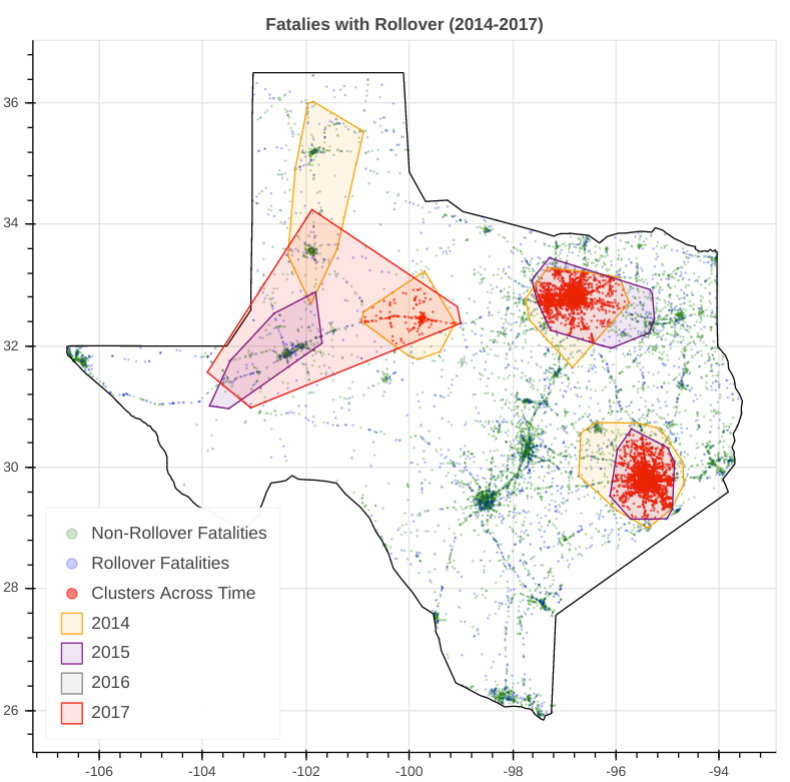
\includegraphics[scale=0.4]{technical.png}
\end{center}
From the map above, there appears to be a cluster in a rural flat area in West Texas. The West Texas area is extremely flat and low density, the cluster appearance is unexpected. Since rollovers are likely to require high speeds in flat areas, a hypothesis of excessive speeding in the area may be further examined. This can easily be contrasted with the more urban Austin area, which is hilly, higher density and does not have any rollover clusters.


\bibliographystlye{apacite}
\bibliography{References}

\end{document}
